\ifx\engineeringnotes\undefined
    \providecommand{\notesroot}{../..}
    \providecommand{\pythonroot}{.}

    \title{Python}
    \author{Donald Cheung\\jianzhang9102@gmail.com}
    \date{\today\footnote{文档编写开始于2018年05月09日}}

    \documentclass[a4paper,10pt]{ctexbook}
\usepackage{xeCJK}
\usepackage{fontspec}
\usepackage{minted}
\usepackage[CJKbookmarks,colorlinks,linkcolor=red]{hyperref}
\usepackage{geometry}
\usepackage{amsmath}
\usepackage[format=hang,font=small,textfont=it]{caption}
\usepackage{float}
\usepackage{subfigure}
\usepackage[nottoc]{tocbibind}
\usepackage{bm}
\usepackage[table, x11names, dvipsnames]{xcolor}
\usepackage{color}
\usepackage{array, booktabs, boldline}
\usepackage{cellspace}
\usepackage{longtable}

\setmainfont{Times New Roman}
\setsansfont{Helvetica}
\setmonofont{Courier New}
\setCJKmainfont[BoldFont={SimHei},ItalicFont={SimHei}]{SimSun}
\setCJKsansfont{SimSun}
\setCJKmonofont{SimSun}

\setcounter{secnumdepth}{4}
\setcounter{tocdepth}{4}

\geometry{left=3.0cm,right=3.0cm,top=2.5cm,bottom=2.5cm}
\bibliographystyle{plain}

%%%%%%%%%%%%%%%%%%%%%%%%%%%%%%%%% minted setting %%%%%%%%%%%%%%%%%%%%%%%%%%%%%%%%%%%
\usemintedstyle{monokai}
\definecolor{bg}{HTML}{282828} % from https://github.com/kevinsawicki/monokai
%\defaultfontfeatures{}
\newfontfamily\noligsmonofamily[NFSSFamily=noligsmonofamily]{Courier}
\setminted{fontfamily=noligsmonofamily}

\renewcommand{\theFancyVerbLine}{%
    \sffamily \textcolor{Dandelion}{\scriptsize \oldstylenums{\arabic{FancyVerbLine}}}}

\newenvironment{jcode}[3]
{%
    \VerbatimEnvironment
    \begin{listing}[h]%
    \caption{#2}%
    \label{#3}%
    \begin{minted}[xleftmargin=18pt,
                   mathescape,
                   linenos,
                   numbersep=5pt,
                   bgcolor=bg,
                   frame=lines,
                   framesep=2mm,
                   fontsize=\footnotesize]{#1}%
}
{%
    \end{minted}
    \vspace{-25pt}%
    \end{listing}%
}
\renewcommand{\listingscaption}{代码}%from minted
\renewcommand{\listoflistingscaption}{代码列表}% from minted


\newenvironment{myquote}{\begin{quote}\kaishu\zihao{-5}}{\end{quote}}
\newcommand\degree{^\circ}
\newtheorem{thm}{定理}


\begin{document}
\maketitle
\tableofcontents
\listoflistings

\else
    \providecommand{\pythonroot}{\engineeringroot/Python}
\fi

\chapter{Python}

\section{Python安装}

可以通过 python/lib/site-package/myconfig.pth 类似的文件类配置Python的额外库的搜索路径。


\section{字符串编码}
字符串也是一种数据类型,但是,字符串比较特殊的是还有一个编码问题。

因为计算机只能处理数字,如果要处理文本,就必须先把文本转换为数字才能处理。最早的计算机在设计时采用8个比特(bit)作为一个字节(byte),所以,一个字节能表示的最大的整数就是255(二进制11111111=十进制255),如果要表示更大的整数,就必须用更多的字节。比如两个字节可以表示的最大整数是65535,4个字节可以表示的最大整数是4294967295。

由于计算机是美国人发明的,因此,最早只有127个字母被编码到计算机里,也就是大小写英文字母、数字和一些符号,这个编码表被称为ASCII编码,比如大写字母A的编码是65,小写字母z的编码是122。

但是要处理中文显然一个字节是不够的,至少需要两个字节,而且还不能和ASCII编码冲突,所以,中国制定了GB2312编码,用来把中文编进去。

你可以想得到的是,全世界有上百种语言,日本把日文编到Shift\_JIS里,韩国把韩文编到Euc-kr里,各国有各国的标准,就会不可避免地出现冲突,结果就是,在多语言混合的文本中,显示出来会有乱码。

因此,Unicode应运而生。Unicode把所有语言都统一到一套编码里,这样就不会再有乱码问题了。

Unicode标准也在不断发展,但最常用的是用两个字节表示一个字符(如果要用到非常偏僻的字符,就需要4个字节)。现代操作系统和大多数编程语言都直接支持Unicode。

现在,捋一捋ASCII编码和Unicode编码的区别:ASCII编码是1个字节,而Unicode编码通常是2个字节。

字母A用ASCII编码是十进制的65,二进制的01000001;

字符0用ASCII编码是十进制的48,二进制的00110000,注意字符'0'和整数0是不同的;

汉字中已经超出了ASCII编码的范围,用Unicode编码是十进制的20013,二进制的01001110 00101101。

你可以猜测,如果把ASCII编码的A用Unicode编码,只需要在前面补0就可以,因此,A的Unicode编码是00000000 01000001。

新的问题又出现了:如果统一成Unicode编码,乱码问题从此消失了。但是,如果你写的文本基本上全部是英文的话,用Unicode编码比ASCII编码需要多一倍的存储空间,在存储和传输上就十分不划算。

所以,本着节约的精神,又出现了把Unicode编码转化为“可变长编码”的UTF-8编码。UTF-8编码把一个Unicode字符根据不同的数字大小编码成1-6个字节,常用的英文字母被编码成1个字节,汉字通常是3个字节,只有很生僻的字符才会被编码成4-6个字节。如果你要传输的文本包含大量英文字符,用UTF-8编码就能节省空间:

字符	ASCII	Unicode	UTF-8
A	01000001	00000000 01000001	01000001
中	x	01001110 00101101	11100100 10111000 10101101
从上面的表格还可以发现,UTF-8编码有一个额外的好处,就是ASCII编码实际上可以被看成是UTF-8编码的一部分,所以,大量只支持ASCII编码的历史遗留软件可以在UTF-8编码下继续工作。

搞清楚了ASCII、Unicode和UTF-8的关系,我们就可以总结一下现在计算机系统通用的字符编码工作方式:

在计算机内存中,统一使用Unicode编码,当需要保存到硬盘或者需要传输的时候,就转换为UTF-8编码。

用记事本编辑的时候,从文件读取的UTF-8字符被转换为Unicode字符到内存里,编辑完成后,保存的时候再把Unicode转换为UTF-8保存到文件:

rw-file-utf-8

浏览网页的时候,服务器会把动态生成的Unicode内容转换为UTF-8再传输到浏览器:

web-utf-8

所以你看到很多网页的源码上会有类似<meta charset="UTF-8" />的信息,表示该网页正是用的UTF-8编码。






\subsection{}

\subsection{Python字符串编码}
%有人此时会问,我用 print 语句打印出来怎么是乱码或者是中文,并不是字节序列。这是因为你调用 print 语句的时候,默认进行了隐式解码,为的是让人类看见友好的字符数据 ,也就是默认的进行了str()包装,想看见背后真正的十六进制数,你需要调用魔术方法 _repr_() 。


\section{常用内置库}
\subsection{logging}


\section{常用第三方库}
%\newpage
\subsection{YAML}
github主页:\href{https://github.com/yaml}{The YAML Project}

假设你有一个YAML配置文件,其内容如\ref{code:yaml-simple-config}所示。

\begin{jcode}{yaml}{YAML代码示例}{code:yaml-simple-config}
# tree format
treeroot:
    branch1:
        name: Node 1
        branch1-1:
            name: Node 1-1
    branch2:
        name: Node 2
        branch2-1:
            name: Node 2-1
\end{jcode}

可以通过\ref{code:yaml-simple-usage}的代码获取配置文件的内容。

\begin{jcode}{python}{YAML代码示例}{code:yaml-simple-usage}
import yaml
with open('config.yaml') as f:
    # use safe_load instead load
    conf = yaml.safe_load(f)
\end{jcode}

如果想要将现有的项保存成 YAML 文件,则可以采用类似于 \ref{code:yaml-simple-saving} 的代码。
\begin{jcode}{python}{保存配置到YAML文件中}{code:yaml-simple-saving}
with open('config.yaml', "w") as f:
    yaml.dump(conf, f)
\end{jcode}


\subsection{requests}

\chapter{Python}

\begin{itemize}
\item \href{http://www.dengfeilong.com/post/60.html}{python编程中的if \_\_name\_\_ == 'main': 的作用和原理}
\end{itemize}

Python是一种计算机程序设计语言。你可能已经听说过很多种流行的编程语言,比如非常难学的C语言,非常流行的Java语言,适合初学者的Basic语言,适合网页编程的JavaScript语言等等。

那Python是一种什么语言?

首先,我们普及一下编程语言的基础知识。用任何编程语言来开发程序,都是为了让计算机干活,比如下载一个MP3,编写一个文档等等,而计算机干活的CPU只认识机器指令,所以,尽管不同的编程语言差异极大,最后都得``翻译"成CPU可以执行的机器指令。而不同的编程语言,干同一个活,编写的代码量,差距也很大。

比如,完成同一个任务,C语言要写1000行代码,Java只需要写100行,而Python可能只要20行。

所以Python是一种相当高级的语言。

你也许会问,代码少还不好?代码少的代价是运行速度慢,C程序运行1秒钟,Java程序可能需要2秒,而Python程序可能就需要10秒。

那是不是越低级的程序越难学,越高级的程序越简单?表面上来说,是的,但是,在非常高的抽象计算中,高级的Python程序设计也是非常难学的,所以,高级程序语言不等于简单。

但是,对于初学者和完成普通任务,Python语言是非常简单易用的。连Google都在大规模使用Python,你就不用担心学了会没用。

用Python可以做什么?可以做日常任务,比如自动备份你的MP3;可以做网站,很多著名的网站包括YouTube就是Python写的;可以做网络游戏的后台,很多在线游戏的后台都是Python开发的。总之就是能干很多很多事啦。

Python当然也有不能干的事情,比如写操作系统,这个只能用C语言写;写手机应用,只能用Objective-C(针对iPhone)和Java(针对Android);写3D游戏,最好用C或C++。

\section{Python简介}
\subsection{Python是什么}
Python是著名的``龟叔" Guido van Rossum在1989年圣诞节期间,为了打发无聊的圣诞节而编写的一个编程语言。

现在,全世界差不多有600多种编程语言,但流行的编程语言也就那么20来种。有很多衡量编程语言流行度的方法,比较出名的有TIOBE编程语言排行榜(\ref{fig:TIOBE_INDEX_2017}、\ref{fig:TIOBE_Index_for_January_2017}、\ref{fig:TIOBE_Top10_LANGUAGE_EVOLUTION})、PYPL编程语言人气指数(\ref{fig:PYPL_INDEX_2017}、\ref{fig:PYPL_PopularitY_of_Programming_Language})、RedMonk编程语言排行榜(\ref{fig:REDMONK_RANKING_2017})\footnote{参考链接:\href{https://www.codingame.com/blog/top-programming-languages-to-learn-in-2017/}{TOP PROGRAMMING LANGUAGES TO LEARN IN 2017}}。

\begin{figure}[ht]
  \centering
  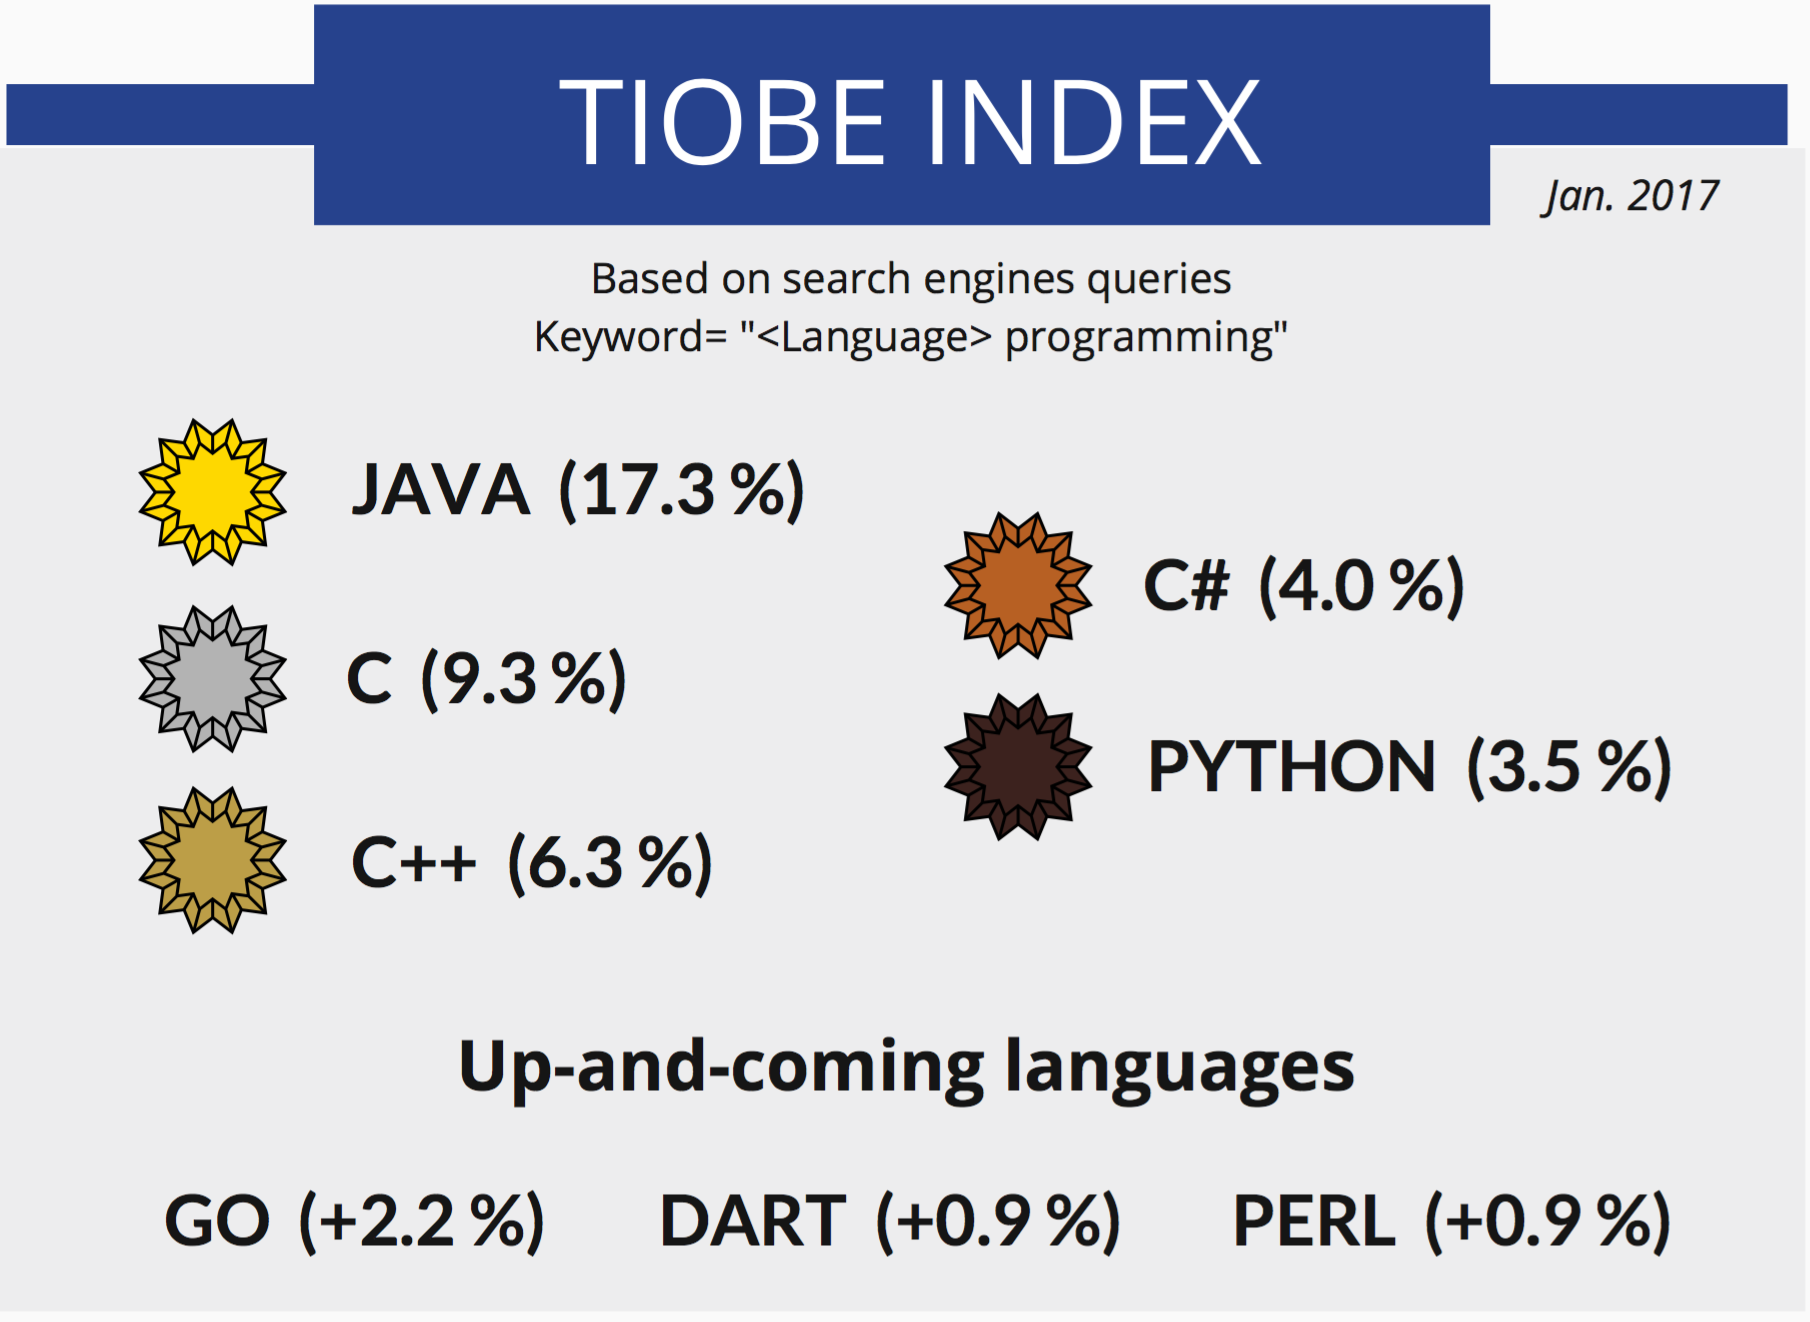
\includegraphics[scale=0.3]{\pythonroot/images/TIOBE_INDEX_2017.png}
  \caption{2017年TIOBE编程语言排行榜}
  \label{fig:TIOBE_INDEX_2017}
\end{figure}

\begin{figure}[ht]
  \centering
  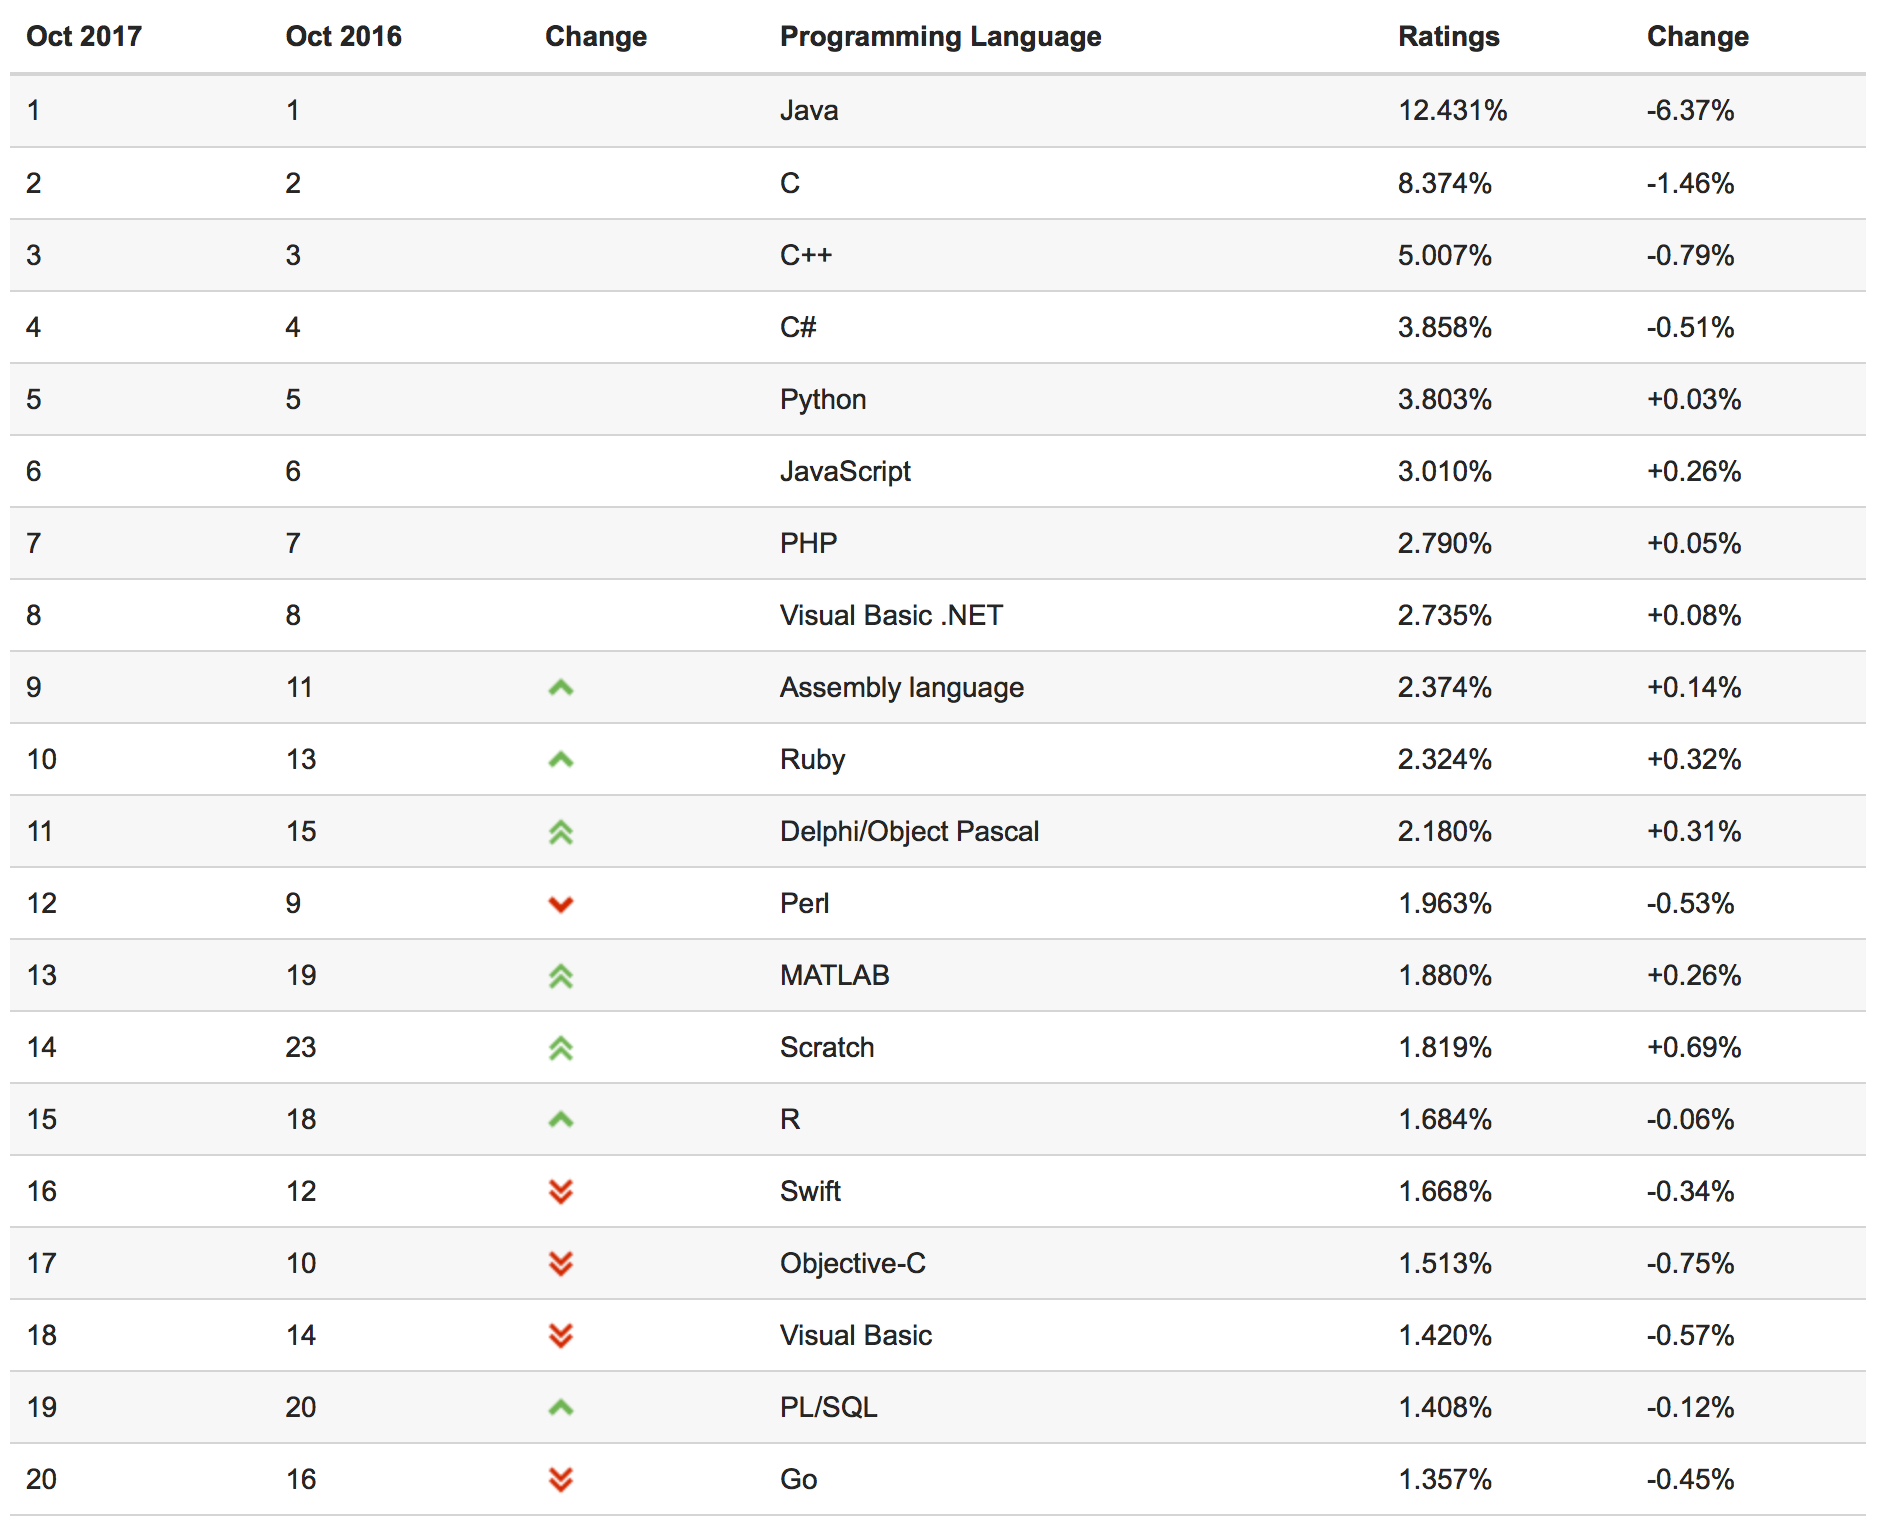
\includegraphics[scale=0.4]{\pythonroot/images/TIOBE_Index_for_January_2017.png}
  \caption{2017年1月TIOBE编程语言排行榜,来源:\href{http://www.tiobe.com/tiobe-index//}{TIOBE Index for January 2017}}
  \label{fig:TIOBE_Index_for_January_2017}
\end{figure}

\begin{figure}[ht]
  \centering
  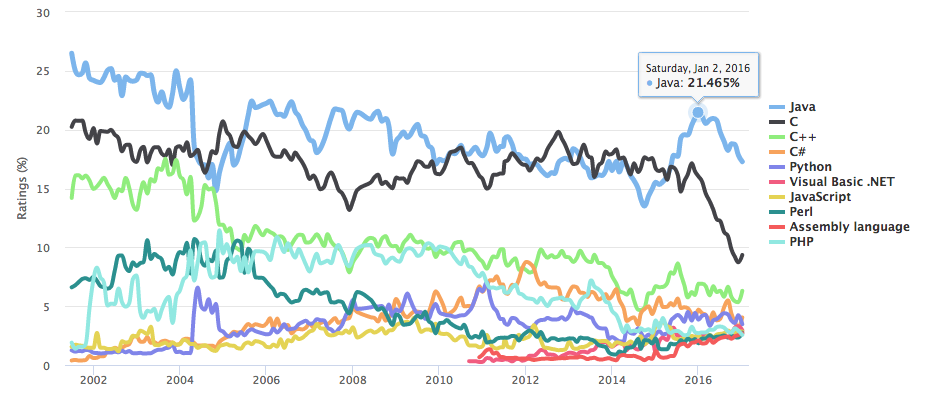
\includegraphics[scale=0.5]{\pythonroot/images/Evolution_of_the_top_10_languages_according_to_Tiobe.png}
  \caption{2017年TIOBE十大编程语言的演变,来源:\href{http://www.tiobe.com/tiobe-index//}{TIOBE Index for January 2017}}
  \label{fig:TIOBE_Top10_LANGUAGE_EVOLUTION}
\end{figure}

\begin{figure}[ht]
  \centering
  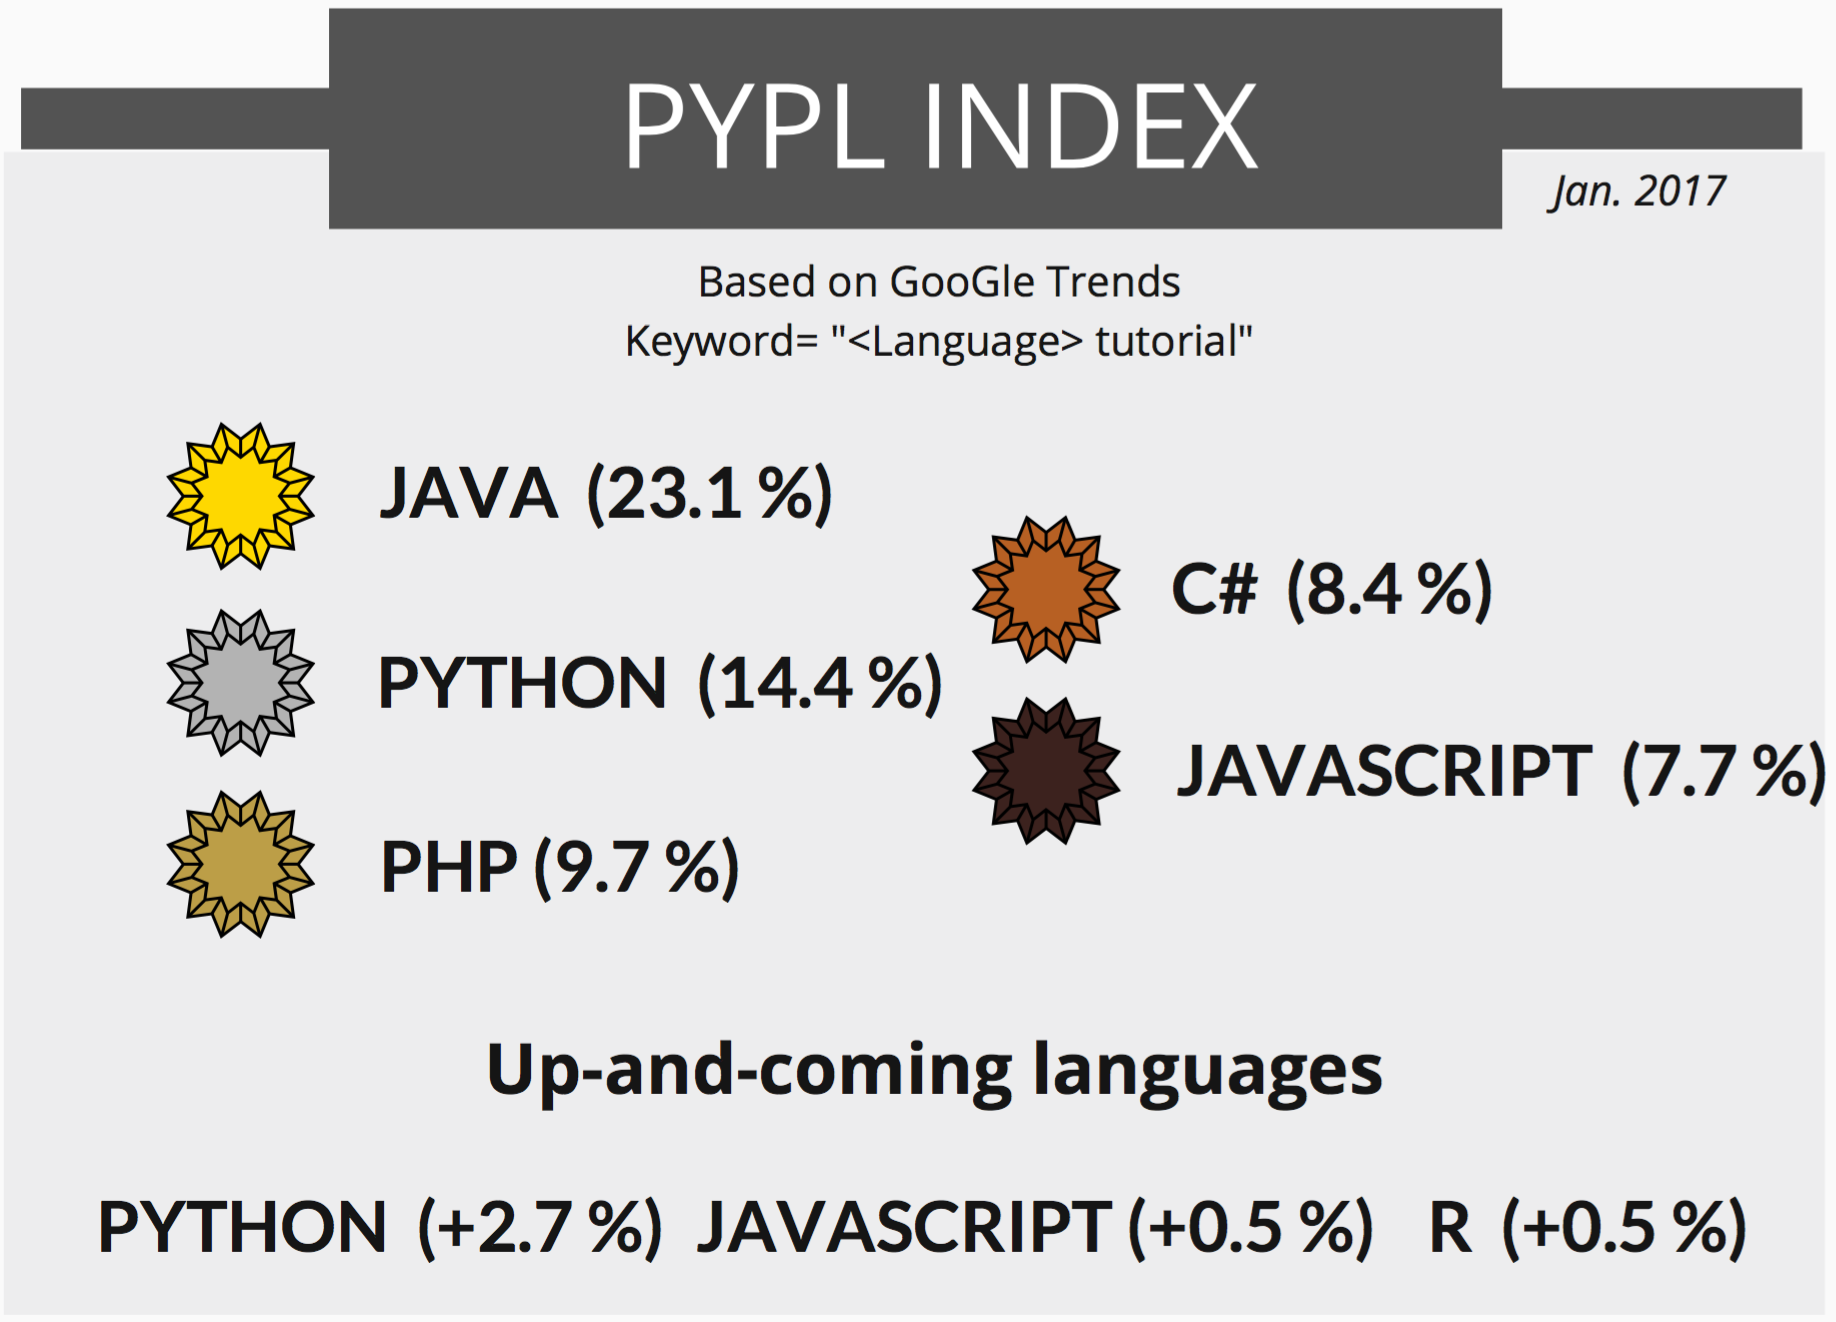
\includegraphics[scale=0.3]{\pythonroot/images/PYPL_INDEX_2017.png}
  \caption{2017年PYPL编程语言人气指数}
  \label{fig:PYPL_INDEX_2017}
\end{figure}

\begin{figure}[ht]
  \centering
  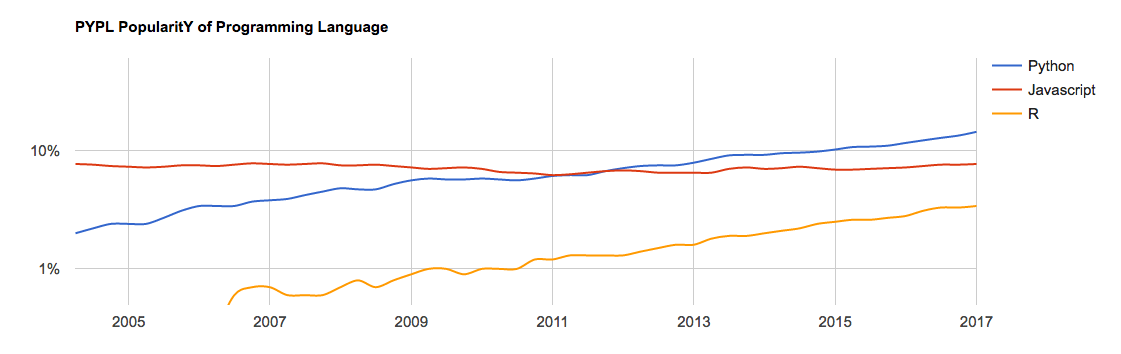
\includegraphics[scale=0.4]{\pythonroot/images/PYPL_PopularitY_of_Programming_Language.png}
  \caption{2017年PYPL编程语言人气指数,来源:\href{http://pypl.github.io/PYPL.html}{PYPL PopularitY of Programming Language Index, January 2017}}
  \label{fig:PYPL_PopularitY_of_Programming_Language}
\end{figure}


\begin{figure}[ht]
  \centering
  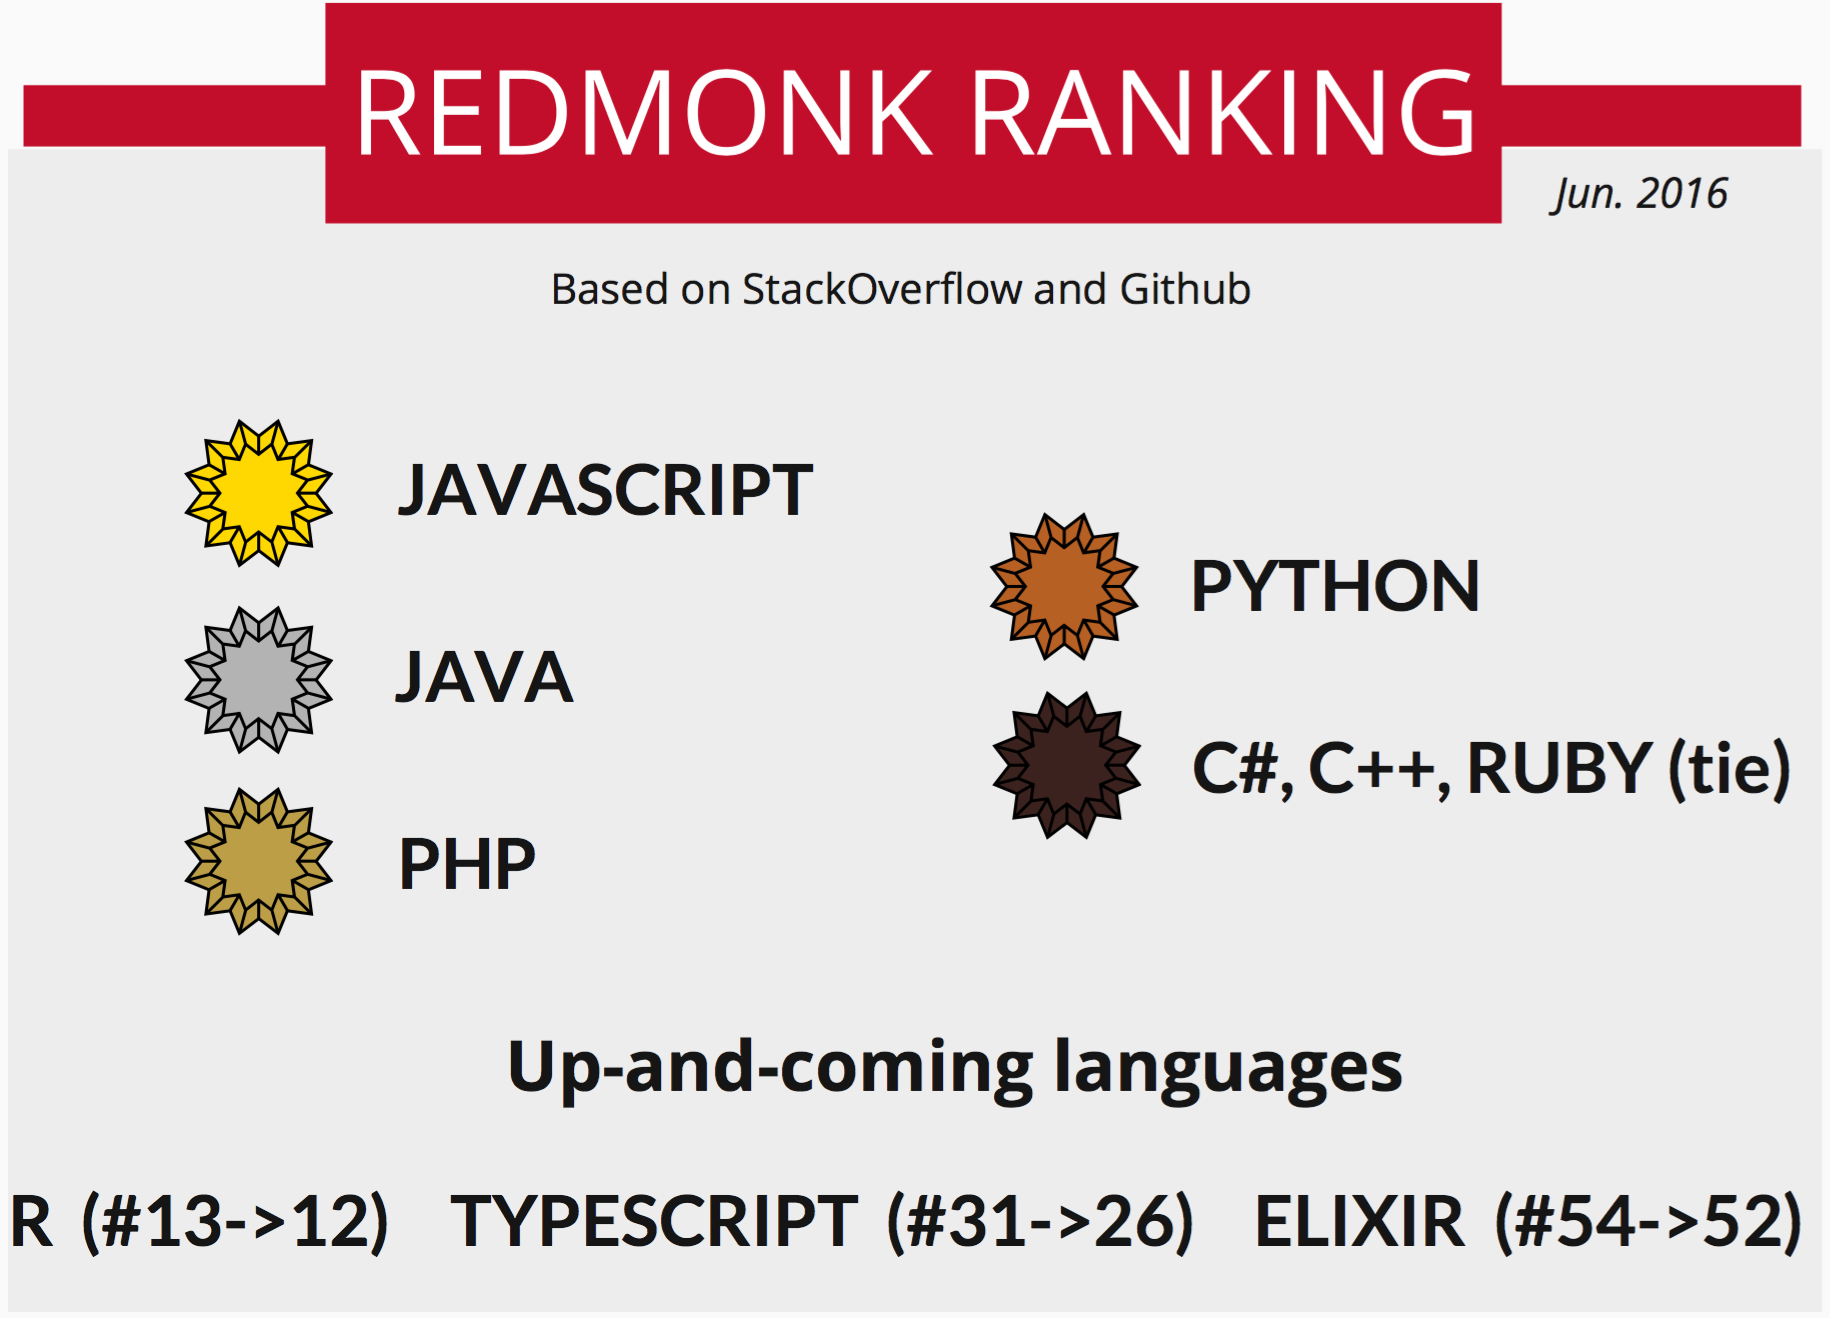
\includegraphics[scale=0.3]{\pythonroot/images/REDMONK_RANKING_2017.png}
  \caption{RedMonk编程语言排行榜}
  \label{fig:REDMONK_RANKING_2017}
\end{figure}

总的来说,这几种编程语言各有千秋。C语言是可以用来编写操作系统的贴近硬件的语言,所以,C语言适合开发那些追求运行速度、充分发挥硬件性能的程序。而Python是用来编写应用程序的高级编程语言。

当你用一种语言开始作真正的软件开发时,你除了编写代码外,还需要很多基本的已经写好的现成的东西,来帮助你加快开发进度。比如说,要编写一个电子邮件客户端,如果先从最底层开始编写网络协议相关的代码,那估计一年半载也开发不出来。高级编程语言通常都会提供一个比较完善的基础代码库,让你能直接调用,比如,针对电子邮件协议的SMTP库,针对桌面环境的GUI库,在这些已有的代码库的基础上开发,一个电子邮件客户端几天就能开发出来。

Python就为我们提供了非常完善的基础代码库,覆盖了网络、文件、GUI、数据库、文本等大量内容,被形象地称作``内置电池(batteries included)"。用Python开发,许多功能不必从零编写,直接使用现成的即可。

除了内置的库外,Python还有大量的第三方库,也就是别人开发的,供你直接使用的东西。当然,如果你开发的代码通过很好的封装,也可以作为第三方库给别人使用。

许多大型网站就是用Python开发的,例如YouTube、Instagram,还有国内的豆瓣。很多大公司,包括Google、Yahoo等,甚至NASA(美国航空航天局)都大量地使用Python。

龟叔给Python的定位是``优雅"、``明确"、``简单",所以Python程序看上去总是简单易懂,初学者学Python,不但入门容易,而且将来深入下去,可以编写那些非常非常复杂的程序。

总的来说,Python的哲学就是简单优雅,尽量写容易看明白的代码,尽量写少的代码。如果一个资深程序员向你炫耀他写的晦涩难懂、动不动就几万行的代码,你可以尽情地嘲笑他。

那Python适合开发哪些类型的应用呢?

首选是网络应用,包括网站、后台服务等等;

其次是许多日常需要的小工具,包括系统管理员需要的脚本任务等等;

另外就是把其他语言开发的程序再包装起来,方便使用。

最后说说Python的缺点。

任何编程语言都有缺点,Python也不例外。优点说过了,那Python有哪些缺点呢?

第一个缺点就是运行速度慢,和C程序相比非常慢,因为Python是解释型语言,你的代码在执行时会一行一行地翻译成CPU能理解的机器码,这个翻译过程非常耗时,所以很慢。而C程序是运行前直接编译成CPU能执行的机器码,所以非常快。

但是大量的应用程序不需要这么快的运行速度,因为用户根本感觉不出来。例如开发一个下载MP3的网络应用程序,C程序的运行时间需要0.001秒,而Python程序的运行时间需要0.1秒,慢了100倍,但由于网络更慢,需要等待1秒,你想,用户能感觉到1.001秒和1.1秒的区别吗?这就好比F1赛车和普通的出租车在北京三环路上行驶的道理一样,虽然F1赛车理论时速高达400公里,但由于三环路堵车的时速只有20公里,因此,作为乘客,你感觉的时速永远是20公里。

不要在意程序运行速度

第二个缺点就是代码不能加密。如果要发布你的Python程序,实际上就是发布源代码,这一点跟C语言不同,C语言不用发布源代码,只需要把编译后的机器码(也就是你在Windows上常见的xxx.exe文件)发布出去。要从机器码反推出C代码是不可能的,所以,凡是编译型的语言,都没有这个问题,而解释型的语言,则必须把源码发布出去。

这个缺点仅限于你要编写的软件需要卖给别人挣钱的时候。好消息是目前的互联网时代,靠卖软件授权的商业模式越来越少了,靠网站和移动应用卖服务的模式越来越多了,后一种模式不需要把源码给别人。

再说了,现在如火如荼的开源运动和互联网自由开放的精神是一致的,互联网上有无数非常优秀的像Linux一样的开源代码,我们千万不要高估自己写的代码真的有非常大的``商业价值"。那些大公司的代码不愿意开放的更重要的原因是代码写得太烂了,一旦开源,就没人敢用他们的产品了。

当然,Python还有其他若干小缺点,请自行忽略,就不一一列举了。

\subsection{安装Python}
因为Python是跨平台的,它可以运行在Windows、Mac和各种Linux/Unix系统上。在Windows上写Python程序,放到Linux上也是能够运行的。

要开始学习Python编程,首先就得把Python安装到你的电脑里。安装后,你会得到Python解释器(就是负责运行Python程序的),一个命令行交互环境,还有一个简单的集成开发环境。

目前,Python有两个版本,一个是2.x版,一个是3.x版,这两个版本是不兼容的,因为现在Python正在朝着3.x版本进化,在进化过程中,大量的针对2.x版本的代码要修改后才能运行,所以,目前有许多第三方库还暂时无法在3.x上使用。

\section{Python基础}
\subsection{第一个Python程序}
在交互式环境的提示符>>>下,直接输入代码,按回车,就可以立刻得到代码执行结果。
\begin{minted}[mathescape,
               numbersep=5pt,
               frame=lines,
               framesep=2mm]{python}
Python 2.7.12 (default, Dec  1 2016, 20:44:50) 
[GCC 4.2.1 Compatible Apple LLVM 8.0.0 (clang-800.0.42.1)] on darwin
Type "help", "copyright", "credits" or "license" for more information.
>>> print 'Hello World'
Hello World
>>> print('Hello World')
Hello World
\end{minted}

也可以将代码保存在脚本文件中,然后调用python解析器来执行程序。
\begin{minted}[mathescape,
               numbersep=5pt,
               frame=lines,
               framesep=2mm]{python}
$ cat script.py
print 'Hello World'
print('Hello World')

$ python script.py
Hello World
Hello World
\end{minted}

\subsection{Python缩进}
缩进的语句视为代码块,缩进有利有弊。好处是强迫你写出格式化的代码,但没有规定缩进是几个空格还是Tab。按照约定俗成的管理,应该始终坚持使用4个空格的缩进。

缩进的另一个好处是强迫你写出缩进较少的代码,你会倾向于把一段很长的代码拆分成若干函数,从而得到缩进较少的代码。

缩进的坏处就是“复制-粘贴”功能失效了,这是最坑爹的地方。当你重构代码时,粘贴过去的代码必须重新检查缩进是否正确。此外,IDE很难像格式化Java代码那样格式化Python代码。


\subsection{Python标识符}
在Python里,标识符由字母、数字、下划线组成,区分大小写并且不能以数字开头。以下划线开头的标识符是有特殊意义的。以单下划线开头\_foo的代表不能直接访问的类属性,需通过类提供的接口进行访问,不能用from xxx import * 而导入;以双下划线开头的 \_\_foo 代表类的私有成员;以双下划线开头和结尾的 \_\_foo\_\_ 代表 Python 里特殊方法专用的标识,如 \_\_init\_\_() 代表类的构造函数。

Python可以同一行显示多条语句,方法是用分号 ; 分开,如:
\begin{minted}[mathescape,
               numbersep=5pt,
               frame=lines,
               framesep=2mm]{python}
>>> print('hello');print('runoob');
hello
runoob
\end{minted}

\subsection{Python注释}
Python的单行注释使用\#,多行注释采用'''或者""",例如:
\begin{minted}[mathescape,
               linenos,
               numbersep=5pt,
               frame=lines,
               framesep=2mm]{python}
# coding: utf8
# 文件名:test.py

# 第一个注释
print("Hello World")  # 第二个注释
\end{minted}

\begin{minted}[mathescape,
               numbersep=5pt,
               framesep=2mm]{python}
$ python test.py
Hello World
$ 
\end{minted}


\begin{minted}[mathescape,
               %linenos,
               numbersep=5pt,
               frame=lines,
               framesep=2mm]{python}
# coding: utf8
# 文件名:test.py

'''
这是多行注释,使用单引号。
这是多行注释,使用单引号。
这是多行注释,使用单引号。
'''

"""
这是多行注释,使用双引号。
这是多行注释,使用双引号。
这是多行注释,使用双引号。
"""
\end{minted}

\subsection{Python数据类型}
\subsubsection{字符串}
\begin{minted}[mathescape,
               %linenos,
               numbersep=5pt,
               frame=lines,
               framesep=2mm]{python}

>>> s = 'Hello World'
>>> print(s)           # 输出完整字符串
Hello World
>>> print(s[0])        # 输出字符串中的第一个字符
H
>>> print(s[2:5])      # 输出字符串中第三个至第五个之间的字符串
llo
>>> print(s[2:])       # 输出从第三个字符开始的字符串
llo World
>>> print(s * 2)       # 输出字符串两次
Hello WorldHello World
>>> print(s + "TEST")  # 输出连接的字符串
Hello WorldTEST
\end{minted}

\begin{minted}[mathescape,
               %linenos,
               numbersep=5pt,
               frame=lines,
               framesep=2mm]{python}
from __future__ import division
from __future__ import print_function
...
\end{minted}



\subsubsection{列表}
\begin{minted}[mathescape,
               %linenos,
               numbersep=5pt,
               frame=lines,
               framesep=2mm]{python}

>>> lt = ['runoob', 786, 2.23, 'john', 70.2]
>>> tinylist = [123, 'john']
>>> print(lt)               # 输出完整列表
['runoob', 786, 2.23, 'john', 70.2]
>>> print(lt[0])            # 输出列表的第一个元素
runoob
>>> print(lt[1:3])          # 输出第二个至第三个的元素 
[786, 2.23]
>>> print(lt[2:])           # 输出从第三个开始至列表末尾的所有元素
[2.23, 'john', 70.2]
>>> print(tinylist * 2)     # 输出列表两次
[123, 'john', 123, 'john']
>>> print(lt + tinylist)    # 打印组合的列表
['runoob', 786, 2.23, 'john', 70.2, 123, 'john']
\end{minted}

\subsubsection{字典}
\begin{minted}[mathescape, numbersep=5pt, frame=lines, framesep=2mm]{python}
>>> d = {}
>>> d['one'] = "This is one"
>>> d[2] = "This is two"
>> tinydict = {'name': 'john','code':6734, 'dept': 'sales'}
>>> print(d['one'])          # 输出键为'one' 的值
This is one
>>> print(d[2])              # 输出键为 2 的值
This is two
>>> print(tinydict)          # 输出完整的字典
{'dept': 'sales', 'code': 6734, 'name': 'john'}
>>> print(tinydict.keys())   # 输出所有键
['dept', 'code', 'name']
>>> print(tinydict.values()) # 输出所有值
['sales', 6734, 'john']
\end{minted}

\subsubsection{循环控制语句}

\begin{minted}[mathescape, numbersep=5pt, frame=lines, framesep=2mm]{python}
if 判断条件一:
    执行语句一 ...
elif 判断条件二:
    执行语句二 ...
else:
    执行语句三 ...
\end{minted}

\begin{minted}[mathescape, numbersep=5pt, frame=lines, framesep=2mm]{python}
while 判断条件:
    执行语句……
\end{minted}

\begin{minted}[mathescape, numbersep=5pt, frame=lines, framesep=2mm]{python}
for iterating_var in sequence:
    statements(s)
\end{minted}

\subsubsection{函数定义}
你可以定义一个由自己想要功能的函数,以下是简单的规则:
\begin{itemize}
\item 函数代码块以 def 关键词开头,后接函数标识符名称和圆括号()。
\item 任何传入参数和自变量必须放在圆括号中间。圆括号之间可以用于定义参数。
\item 函数的第一行语句可以选择性地使用文档字符串—用于存放函数说明。
\item 函数内容以冒号起始,并且缩进。
\item return [表达式] 结束函数,选择性地返回一个值给调用方。不带表达式的return相当于返回 None。
\end{itemize}

\begin{minted}[mathescape, numbersep=5pt, frame=lines, framesep=2mm]{python}
def functionname(parameters):
    "函数_文档字符串"
    function_suite
    return [expression]
\end{minted}

\subsubsection{特殊函数}
Python内置了一些特殊函数,这些函数很具python特性。可以让代码更加简洁。

\begin{enumerate}
\item filter(function, sequence):
\begin{minted}[mathescape, numbersep=5pt, frame=lines, framesep=2mm]{python}
# Python 2
s = ['a', 'b', 'c', 'd']
def fun1(s):
    return True if s != 'a' else False
ret = filter(fun1, s)
print(ret)
## ['b', 'c', 'd']
\end{minted}

\begin{minted}[mathescape, numbersep=5pt, frame=lines, framesep=2mm]{python}
# Python 3
s = ['a', 'b', 'c', 'd']
def fun1(s):
    return True if s != 'a' else False
ret = filter(fun1, s)
print(ret)
# <filter object at 0x106490940>
print(list(ret))
## ['b', 'c', 'd']
\end{minted}

对sequence中的item依次执行function(item),将执行结果为True的item组成一个List/String/Tuple(取决于sequence的类型)返回。
可以看作是过滤函数。

\item map(function, sequence) 
\begin{minted}[mathescape, numbersep=5pt, frame=lines, framesep=2mm]{python}
# Python 2
s = ['a', 'b', 'c', 'd'] 
def fun2(s):
    return s + ".txt"
ret = map(fun2, s)
print(ret)
# ['a.txt', 'b.txt', 'c.txt', 'd.txt']
\end{minted}


\newpage
\begin{minted}[mathescape, numbersep=5pt, frame=lines, framesep=2mm]{python}
# Python 3
s = ['a', 'b', 'c', 'd'] 
def fun2(s):
    return s + ".txt"
ret = map(fun2, s)
print(ret)
# <map object at 0x10449ea58>
print(list(ret))
# ['a.txt', 'b.txt', 'c.txt', 'd.txt']
\end{minted}

对sequence中的item依次执行function(item),见执行结果组成一个List返回:

map也支持多个sequence,这就要求function也支持相应数量的参数输入:
\begin{minted}[mathescape, numbersep=5pt, frame=lines, framesep=2mm]{python}
def add(x, y):
    return x + y 

print map(add, range(10), range(10)) 
##[0, 2, 4, 6, 8, 10, 12, 14, 16, 18]
\end{minted}

\item reduce(function, sequence, starting\_value)
\begin{minted}[mathescape, numbersep=5pt, frame=lines, framesep=2mm]{python}
from functools import reduce # for python 3
def add1(x,y):
    return x + y
print(reduce(add1, range(1, 100)))
print(reduce(add1, range(1, 100), 20))
# 4950 (注:1+2+...+99)
# 4970 (注:1+2+...+99+20)
\end{minted}

对sequence中的item顺序迭代调用function,如果有starting\_value,还可以作为初始值调用。


\item lambda:
    \newpage
\begin{minted}[mathescape, numbersep=5pt, frame=lines, framesep=2mm]{python}
g = lambda s: s + ".fsh"
print(g("haha"))
print((lambda x: x * 2)(3))

## haha.fsh
## 6
\end{minted}

这是Python支持一种有趣的语法,它允许你快速定义单行的最小函数,类似与C语言中的宏,这些叫做lambda的函数.
\end{enumerate}


\subsection{字符串和编码}

Python的字符串

搞清楚了令人头疼的字符编码问题后,我们再来研究Python对Unicode的支持。

因为Python的诞生比Unicode标准发布的时间还要早,所以最早的Python只支持ASCII编码,普通的字符串'ABC'在Python内部都是ASCII编码的。Python提供了ord()和chr()函数,可以把字母和对应的数字相互转换:

>>> ord('A')
65
>>> chr(65)
'A'
Python在后来添加了对Unicode的支持,以Unicode表示的字符串用u'...'表示,比如:

>>> print u'中文'
中文
>>> u'中'
%u'\u4e2d'
%写u'中'和u'\u4e2d'是一样的,\u后面是十六进制的Unicode码。因此,u'A'和u'\u0041'也是一样的。

两种字符串如何相互转换?字符串'xxx'虽然是ASCII编码,但也可以看成是UTF-8编码,而u'xxx'则只能是Unicode编码。

把u'xxx'转换为UTF-8编码的'xxx'用encode('utf-8')方法:

>>> u'ABC'.encode('utf-8')
'ABC'
>>> u'中文'.encode('utf-8')
%'\xe4\xb8\xad\xe6\x96\x87'
%英文字符转换后表示的UTF-8的值和Unicode值相等(但占用的存储空间不同),而中文字符转换后1个Unicode字符将变为3个UTF-8字符,你看到的\xe4就是其中一个字节,因为它的值是228,没有对应的字母可以显示,所以以十六进制显示字节的数值。len()函数可以返回字符串的长度:

>>> len(u'ABC')
3
>>> len('ABC')
3
>>> len(u'中文')
2
%>>> len('\xe4\xb8\xad\xe6\x96\x87')
6
反过来,把UTF-8编码表示的字符串'xxx'转换为Unicode字符串u'xxx'用decode('utf-8')方法:

>>> 'abc'.decode('utf-8')
u'abc'
%>>> '\xe4\xb8\xad\xe6\x96\x87'.decode('utf-8')
%u'\u4e2d\u6587'
%>>> print '\xe4\xb8\xad\xe6\x96\x87'.decode('utf-8')
中文
由于Python源代码也是一个文本文件,所以,当你的源代码中包含中文的时候,在保存源代码时,就需要务必指定保存为UTF-8编码。当Python解释器读取源代码时,为了让它按UTF-8编码读取,我们通常在文件开头写上这两行:

%#!/usr/bin/env python
%# -*- coding: utf-8 -*-
第一行注释是为了告诉Linux/OS X系统,这是一个Python可执行程序,Windows系统会忽略这个注释;

第二行注释是为了告诉Python解释器,按照UTF-8编码读取源代码,否则,你在源代码中写的中文输出可能会有乱码。

%如果你使用Notepad++进行编辑,除了要加上# -*- coding: utf-8 -*-外,中文字符串必须是Unicode字符串:

申明了UTF-8编码并不意味着你的.py文件就是UTF-8编码的,必须并且要确保Notepad++正在使用UTF-8 without BOM编码:

set-encoding-in-notepad++

%如果.py文件本身使用UTF-8编码,并且也申明了# -*- coding: utf-8 -*-,打开命令提示符测试就可以正常显示中文:

py-chinese-test-in-cmd

格式化

最后一个常见的问题是如何输出格式化的字符串。我们经常会输出类似'亲爱的xxx你好!你xx月的话费是xx,余额是xx'之类的字符串,而xxx的内容都是根据变量变化的,所以,需要一种简便的格式化字符串的方式。

py-str-format

在Python中,采用的格式化方式和C语言是一致的,用%实现,举例如下:

%>>> 'Hello, %s' % 'world'
%'Hello, world'
%>>> 'Hi, %s, you have $%d.' % ('Michael', 1000000)
%'Hi, Michael, you have $1000000.'
你可能猜到了,%运算符就是用来格式化字符串的。在字符串内部,%s表示用字符串替换,%d表示用整数替换,有几个%?占位符,后面就跟几个变量或者值,顺序要对应好。如果只有一个%?,括号可以省略。

常见的占位符有:

%d	整数
%f	浮点数
%s	字符串
%x	十六进制整数
其中,格式化整数和浮点数还可以指定是否补0和整数与小数的位数:

>>> '%2d-%02d' % (3, 1)
' 3-01'
>>> '%.2f' % 3.1415926
'3.14'
如果你不太确定应该用什么,%s永远起作用,它会把任何数据类型转换为字符串:

>>> 'Age: %s. Gender: %s' % (25, True)
'Age: 25. Gender: True'
对于Unicode字符串,用法完全一样,但最好确保替换的字符串也是Unicode字符串:

>>> u'Hi, %s' % u'Michael'
u'Hi, Michael'
有些时候,字符串里面的%是一个普通字符怎么办?这个时候就需要转义,用%%来表示一个%:

>>> 'growth rate: %d %%' % 7
'growth rate: 7 %'
小结

由于历史遗留问题,Python 2.x版本虽然支持Unicode,但在语法上需要'xxx'和u'xxx'两种字符串表示方式。

Python当然也支持其他编码方式,比如把Unicode编码成GB2312:

>>> u'中文'.encode('gb2312')
%'\xd6\xd0\xce\xc4'
但这种方式纯属自找麻烦,如果没有特殊业务要求,请牢记仅使用Unicode和UTF-8这两种编码方式。

在Python 3.x版本中,把'xxx'和u'xxx'统一成Unicode编码,即写不写前缀u都是一样的,而以字节形式表示的字符串则必须加上b前缀:b'xxx'。

格式化字符串的时候,可以用Python的交互式命令行测试,方便快捷。


\subsection{使用list和tuple}

使用list和tuple

Reads: 450657
list

Python内置的一种数据类型是列表:list。list是一种有序的集合,可以随时添加和删除其中的元素。

比如,列出班里所有同学的名字,就可以用一个list表示:

%>>> classmates = ['Michael', 'Bob', 'Tracy']
>>> classmates
%['Michael', 'Bob', 'Tracy']
变量classmates就是一个list。用len()函数可以获得list元素的个数:

>>> len(classmates)
3
用索引来访问list中每一个位置的元素,记得索引是从0开始的:

%>>> classmates[0]
'Michael'
%>>> classmates[1]
'Bob'
%>>> classmates[2]
'Tracy'
%>>> classmates[3]
Traceback (most recent call last):
  File "<stdin>", line 1, in <module>
IndexError: list index out of range
当索引超出了范围时,Python会报一个IndexError错误,所以,要确保索引不要越界,记得最后一个元素的索引是len(classmates) - 1。

如果要取最后一个元素,除了计算索引位置外,还可以用-1做索引,直接获取最后一个元素:

>>> classmates[-1]
'Tracy'
以此类推,可以获取倒数第2个、倒数第3个:

>>> classmates[-2]
'Bob'
>>> classmates[-3]
'Michael'
>>> classmates[-4]
Traceback (most recent call last):
  File "<stdin>", line 1, in <module>
IndexError: list index out of range
当然,倒数第4个就越界了。

list是一个可变的有序表,所以,可以往list中追加元素到末尾:

>>> classmates.append('Adam')
>>> classmates
['Michael', 'Bob', 'Tracy', 'Adam']
也可以把元素插入到指定的位置,比如索引号为1的位置:

>>> classmates.insert(1, 'Jack')
>>> classmates
['Michael', 'Jack', 'Bob', 'Tracy', 'Adam']
要删除list末尾的元素,用pop()方法:

>>> classmates.pop()
'Adam'
>>> classmates
['Michael', 'Jack', 'Bob', 'Tracy']
要删除指定位置的元素,用pop(i)方法,其中i是索引位置:

>>> classmates.pop(1)
'Jack'
>>> classmates
['Michael', 'Bob', 'Tracy']
要把某个元素替换成别的元素,可以直接赋值给对应的索引位置:

>>> classmates[1] = 'Sarah'
>>> classmates
['Michael', 'Sarah', 'Tracy']
list里面的元素的数据类型也可以不同,比如:

>>> L = ['Apple', 123, True]
list元素也可以是另一个list,比如:

>>> s = ['python', 'java', ['asp', 'php'], 'scheme']
>>> len(s)
4
要注意s只有4个元素,其中s[2]又是一个list,如果拆开写就更容易理解了:

>>> p = ['asp', 'php']
>>> s = ['python', 'java', p, 'scheme']
要拿到'php'可以写p[1]或者s[2][1],因此s可以看成是一个二维数组,类似的还有三维、四维……数组,不过很少用到。

如果一个list中一个元素也没有,就是一个空的list,它的长度为0:

>>> L = []
>>> len(L)
0
tuple

另一种有序列表叫元组:tuple。tuple和list非常类似,但是tuple一旦初始化就不能修改,比如同样是列出同学的名字:

>>> classmates = ('Michael', 'Bob', 'Tracy')
现在,classmates这个tuple不能变了,它也没有append(),insert()这样的方法。其他获取元素的方法和list是一样的,你可以正常地使用classmates[0],classmates[-1],但不能赋值成另外的元素。

不可变的tuple有什么意义?因为tuple不可变,所以代码更安全。如果可能,能用tuple代替list就尽量用tuple。

tuple的陷阱:当你定义一个tuple时,在定义的时候,tuple的元素就必须被确定下来,比如:

>>> t = (1, 2)
>>> t
(1, 2)
如果要定义一个空的tuple,可以写成():

>>> t = ()
>>> t
()
但是,要定义一个只有1个元素的tuple,如果你这么定义:

>>> t = (1)
>>> t
1
定义的不是tuple,是1这个数!这是因为括号()既可以表示tuple,又可以表示数学公式中的小括号,这就产生了歧义,因此,Python规定,这种情况下,按小括号进行计算,计算结果自然是1。

所以,只有1个元素的tuple定义时必须加一个逗号,,来消除歧义:

>>> t = (1,)
>>> t
(1,)
Python在显示只有1个元素的tuple时,也会加一个逗号,,以免你误解成数学计算意义上的括号。

最后来看一个“可变的”tuple:

>>> t = ('a', 'b', ['A', 'B'])
>>> t[2][0] = 'X'
>>> t[2][1] = 'Y'
>>> t
('a', 'b', ['X', 'Y'])
这个tuple定义的时候有3个元素,分别是'a','b'和一个list。不是说tuple一旦定义后就不可变了吗?怎么后来又变了?

别急,我们先看看定义的时候tuple包含的3个元素:

tuple-0

当我们把list的元素'A'和'B'修改为'X'和'Y'后,tuple变为:

tuple-1

表面上看,tuple的元素确实变了,但其实变的不是tuple的元素,而是list的元素。tuple一开始指向的list并没有改成别的list,所以,tuple所谓的“不变”是说,tuple的每个元素,指向永远不变。即指向'a',就不能改成指向'b',指向一个list,就不能改成指向其他对象,但指向的这个list本身是可变的!

理解了“指向不变”后,要创建一个内容也不变的tuple怎么做?那就必须保证tuple的每一个元素本身也不能变。

小结

list和tuple是Python内置的有序集合,一个可变,一个不可变。根据需要来选择使用它们。




\subsection{条件判断和循环}
条件判断

计算机之所以能做很多自动化的任务,因为它可以自己做条件判断。

比如,输入用户年龄,根据年龄打印不同的内容,在Python程序中,用if语句实现:

age = 20
if age >= 18:
    print 'your age is', age
    print 'adult'
根据Python的缩进规则,如果if语句判断是True,就把缩进的两行print语句执行了,否则,什么也不做。

也可以给if添加一个else语句,意思是,如果if判断是False,不要执行if的内容,去把else执行了:

age = 3
if age >= 18:
    print 'your age is', age
    print 'adult'
else:
    print 'your age is', age
    print 'teenager'
注意不要少写了冒号:。

当然上面的判断是很粗略的,完全可以用elif做更细致的判断:

age = 3
if age >= 18:
    print 'adult'
elif age >= 6:
    print 'teenager'
else:
    print 'kid'
elif是else if的缩写,完全可以有多个elif,所以if语句的完整形式就是:

if <条件判断1>:
    <执行1>
elif <条件判断2>:
    <执行2>
elif <条件判断3>:
    <执行3>
else:
    <执行4>
if语句执行有个特点,它是从上往下判断,如果在某个判断上是True,把该判断对应的语句执行后,就忽略掉剩下的elif和else,所以,请测试并解释为什么下面的程序打印的是teenager:

age = 20
if age >= 6:
    print 'teenager'
elif age >= 18:
    print 'adult'
else:
    print 'kid'
if判断条件还可以简写,比如写:

if x:
    print 'True'
只要x是非零数值、非空字符串、非空list等,就判断为True,否则为False。

循环

Python的循环有两种,一种是for...in循环,依次把list或tuple中的每个元素迭代出来,看例子:

names = ['Michael', 'Bob', 'Tracy']
for name in names:
    print name
执行这段代码,会依次打印names的每一个元素:

Michael
Bob
Tracy
所以for x in ...循环就是把每个元素代入变量x,然后执行缩进块的语句。

再比如我们想计算1-10的整数之和,可以用一个sum变量做累加:

sum = 0
for x in [1, 2, 3, 4, 5, 6, 7, 8, 9, 10]:
    sum = sum + x
print sum
如果要计算1-100的整数之和,从1写到100有点困难,幸好Python提供一个range()函数,可以生成一个整数序列,比如range(5)生成的序列是从0开始小于5的整数:

>>> range(5)
[0, 1, 2, 3, 4]
range(101)就可以生成0-100的整数序列,计算如下:

sum = 0
for x in range(101):
    sum = sum + x
print sum
请自行运行上述代码,看看结果是不是当年高斯同学心算出的5050。

第二种循环是while循环,只要条件满足,就不断循环,条件不满足时退出循环。比如我们要计算100以内所有奇数之和,可以用while循环实现:

sum = 0
n = 99
while n > 0:
    sum = sum + n
    n = n - 2
print sum
在循环内部变量n不断自减,直到变为-1时,不再满足while条件,循环退出。

%再议raw_input

%最后看一个有问题的条件判断。很多同学会用raw_input()读取用户的输入,这样可以自己输入,程序运行得更有意思:

%birth = raw_input('birth: ')
if birth < 2000:
    print '00前'
else:
    print '00后'
输入1982,结果却显示00后,这么简单的判断Python也能搞错?

当然不是Python的问题,在Python的交互式命令行下打印birth看看:

>>> birth
'1982'
>>> '1982' < 2000
False
>>> 1982 < 2000
True
%原因找到了!原来从raw_input()读取的内容永远以字符串的形式返回,把字符串和整数比较就不会得到期待的结果,必须先用int()把字符串转换为我们想要的整型:

%birth = int(raw_input('birth: '))
再次运行,就可以得到正确地结果。但是,如果输入abc呢?又会得到一个错误信息:

Traceback (most recent call last):
  ...
ValueError: invalid literal for int() with base 10: 'abc'
原来int()发现一个字符串并不是合法的数字时就会报错,程序就退出了。

如何检查并捕获程序运行期的错误呢?后面的错误和调试会讲到。

小结

条件判断可以让计算机自己做选择,Python的if...elif...else很灵活。

python-if

循环是让计算机做重复任务的有效的方法,有些时候,如果代码写得有问题,会让程序陷入“死循环”,也就是永远循环下去。这时可以用Ctrl+C退出程序,或者强制结束Python进程。


请试写一个死循环程序。






\subsection{使用dict和set}

Reads: 373074
dict

Python内置了字典:dict的支持,dict全称dictionary,在其他语言中也称为map,使用键-值(key-value)存储,具有极快的查找速度。

举个例子,假设要根据同学的名字查找对应的成绩,如果用list实现,需要两个list:

%names = ['Michael', 'Bob', 'Tracy']
%scores = [95, 75, 85]
给定一个名字,要查找对应的成绩,就先要在names中找到对应的位置,再从scores取出对应的成绩,list越长,耗时越长。

如果用dict实现,只需要一个“名字”-“成绩”的对照表,直接根据名字查找成绩,无论这个表有多大,查找速度都不会变慢。用Python写一个dict如下:

%>>> d = {'Michael': 95, 'Bob': 75, 'Tracy': 85}
%>>> d['Michael']
95
为什么dict查找速度这么快?因为dict的实现原理和查字典是一样的。假设字典包含了1万个汉字,我们要查某一个字,一个办法是把字典从第一页往后翻,直到找到我们想要的字为止,这种方法就是在list中查找元素的方法,list越大,查找越慢。

第二种方法是先在字典的索引表里(比如部首表)查这个字对应的页码,然后直接翻到该页,找到这个字,无论找哪个字,这种查找速度都非常快,不会随着字典大小的增加而变慢。

dict就是第二种实现方式,给定一个名字,比如'Michael',dict在内部就可以直接计算出Michael对应的存放成绩的“页码”,也就是95这个数字存放的内存地址,直接取出来,所以速度非常快。

你可以猜到,这种key-value存储方式,在放进去的时候,必须根据key算出value的存放位置,这样,取的时候才能根据key直接拿到value。

把数据放入dict的方法,除了初始化时指定外,还可以通过key放入:

>>> d['Adam'] = 67
>>> d['Adam']
67
由于一个key只能对应一个value,所以,多次对一个key放入value,后面的值会把前面的值冲掉:

>>> d['Jack'] = 90
>>> d['Jack']
90
>>> d['Jack'] = 88
>>> d['Jack']
88
如果key不存在,dict就会报错:

>>> d['Thomas']
Traceback (most recent call last):
  File "<stdin>", line 1, in <module>
KeyError: 'Thomas'
要避免key不存在的错误,有两种办法,一是通过in判断key是否存在:

>>> 'Thomas' in d
False
二是通过dict提供的get方法,如果key不存在,可以返回None,或者自己指定的value:

>>> d.get('Thomas')
>>> d.get('Thomas', -1)
-1
注意:返回None的时候Python的交互式命令行不显示结果。

要删除一个key,用pop(key)方法,对应的value也会从dict中删除:

>>> d.pop('Bob')
75
>>> d
{'Michael': 95, 'Tracy': 85}
请务必注意,dict内部存放的顺序和key放入的顺序是没有关系的。

和list比较,dict有以下几个特点:

查找和插入的速度极快,不会随着key的增加而增加;
需要占用大量的内存,内存浪费多。
而list相反:

查找和插入的时间随着元素的增加而增加;
占用空间小,浪费内存很少。
所以,dict是用空间来换取时间的一种方法。

dict可以用在需要高速查找的很多地方,在Python代码中几乎无处不在,正确使用dict非常重要,需要牢记的第一条就是dict的key必须是不可变对象。

这是因为dict根据key来计算value的存储位置,如果每次计算相同的key得出的结果不同,那dict内部就完全混乱了。这个通过key计算位置的算法称为哈希算法(Hash)。

要保证hash的正确性,作为key的对象就不能变。在Python中,字符串、整数等都是不可变的,因此,可以放心地作为key。而list是可变的,就不能作为key:

>>> key = [1, 2, 3]
>>> d[key] = 'a list'
Traceback (most recent call last):
  File "<stdin>", line 1, in <module>
TypeError: unhashable type: 'list'
set

set和dict类似,也是一组key的集合,但不存储value。由于key不能重复,所以,在set中,没有重复的key。

要创建一个set,需要提供一个list作为输入集合:

>>> s = set([1, 2, 3])
>>> s
set([1, 2, 3])
注意,传入的参数[1, 2, 3]是一个list,而显示的set([1, 2, 3])只是告诉你这个set内部有1,2,3这3个元素,显示的[]不表示这是一个list。

重复元素在set中自动被过滤:

>>> s = set([1, 1, 2, 2, 3, 3])
>>> s
set([1, 2, 3])
通过add(key)方法可以添加元素到set中,可以重复添加,但不会有效果:

>>> s.add(4)
>>> s
set([1, 2, 3, 4])
>>> s.add(4)
>>> s
set([1, 2, 3, 4])
通过remove(key)方法可以删除元素:

>>> s.remove(4)
>>> s
set([1, 2, 3])
set可以看成数学意义上的无序和无重复元素的集合,因此,两个set可以做数学意义上的交集、并集等操作:

>>> s1 = set([1, 2, 3])
>>> s2 = set([2, 3, 4])
%>>> s1 & s2
set([2, 3])
>>> s1 | s2
set([1, 2, 3, 4])
set和dict的唯一区别仅在于没有存储对应的value,但是,set的原理和dict一样,所以,同样不可以放入可变对象,因为无法判断两个可变对象是否相等,也就无法保证set内部“不会有重复元素”。试试把list放入set,看看是否会报错。

再议不可变对象

上面我们讲了,str是不变对象,而list是可变对象。

对于可变对象,比如list,对list进行操作,list内部的内容是会变化的,比如:

>>> a = ['c', 'b', 'a']
>>> a.sort()
>>> a
['a', 'b', 'c']
而对于不可变对象,比如str,对str进行操作呢:

>>> a = 'abc'
>>> a.replace('a', 'A')
'Abc'
>>> a
'abc'
虽然字符串有个replace()方法,也确实变出了'Abc',但变量a最后仍是'abc',应该怎么理解呢?

我们先把代码改成下面这样:

>>> a = 'abc'
>>> b = a.replace('a', 'A')
>>> b
'Abc'
>>> a
'abc'
要始终牢记的是,a是变量,而'abc'才是字符串对象!有些时候,我们经常说,对象a的内容是'abc',但其实是指,a本身是一个变量,它指向的对象的内容才是'abc':

a-to-str

当我们调用a.replace('a', 'A')时,实际上调用方法replace是作用在字符串对象'abc'上的,而这个方法虽然名字叫replace,但却没有改变字符串'abc'的内容。相反,replace方法创建了一个新字符串'Abc'并返回,如果我们用变量b指向该新字符串,就容易理解了,变量a仍指向原有的字符串'abc',但变量b却指向新字符串'Abc'了:

a-b-to-2-strs

所以,对于不变对象来说,调用对象自身的任意方法,也不会改变该对象自身的内容。相反,这些方法会创建新的对象并返回,这样,就保证了不可变对象本身永远是不可变的。

小结

使用key-value存储结构的dict在Python中非常有用,选择不可变对象作为key很重要,最常用的key是字符串。

tuple虽然是不变对象,但试试把(1, 2, 3)和(1, [2, 3])放入dict或set中,并解释结果。


\section{Python装饰器}
If you want to take a really deep dive, you should read these \href{https://github.com/GrahamDumpleton/wrapt/tree/develop/blog}{exhaustive articles} by Graham Dumpleton. However, if you intend to get started and getting better at reading/writing python decorators, this article should suffice.

Everything is an object in python, even functions. A function can be assigned to a variable, passed to another function and can be returned from another function. Take a look at the example below:

\begin{minted}[mathescape,
               numbersep=5pt,
               frame=lines,
               framesep=2mm]{python}
def outer_function():
    print "1. This is outer function!"
    def inner_function():
        print "2. This is inner function, inside outer function!"
    print "3. This is outside inner function, inside outer function!"
    return inner_function()
func_assign = outer_function()

# output:
# 1. This is outer function!
# 3. This is outside inner function, inside outer function!
# 2. This is inner function, inside outer function!
\end{minted}

Mark in the above execution, how the statement inside the inner function is printed at the last, consequential to inner\_function being returned, at the end of outer\_function, and the execution could be seen during the assignment.

Python decorator are the function that receive a function as an argument and return another function as return value. The assumption for a decorator is that we will pass a function as argument and the signature of the inner function in the decorator must match the function to decorate.

装饰器本质上是一个Python函数,它可以让其他函数在不需要做任何代码变动的前提下增加额外功能,装饰器的返回值也是一个函数对象。它经常用于有切面需求的场景,比如:插入日志、性能测试、事务处理、缓存、权限校验等场景。装饰器是解决这类问题的绝佳设计,有了装饰器,我们就可以抽离出大量与函数功能本身无关的雷同代码并继续重用。概括的讲,装饰器的作用就是为已经存在的对象添加额外的功能。

\subsection{函数装饰器}
Let us now, write a simple function decorator for ourselves. We will write a decorator that would measure the execution time of the function passed to it.
\begin{minted}[mathescape,
               numbersep=5pt,
               frame=lines,
               framesep=2mm]{python}
import time
def timetest(input_func):
    def timed(*args, **kwargs):
        start_time = time.time()
        result = input_func(*args, **kwargs)
        end_time = time.time()
        print "Method Name - {0}, Args - {1},\nKwargs - {2}, Time - {3}".format(
                        input_func.__name__, args, kwargs, end_time - start_time)
        return result
    return timed

@timetest
def foobar(*args, **kwargs):
    time.sleep(0.3)
    print "inside foobar"
    print args, kwargs

foobar(["hello"], a=2, b=5)
# output:
# inside foobar
# (['hello'],) {'a': 2, 'b': 5}
# Method Name - foobar, Args - (['hello'],),
# Kwargs - {'a': 2, 'b': 5}, Time - 0.30296087265
\end{minted}

We passed the function foobar to decorator named timetest. Inside decorator, function foobar is referenced as variable input\_func. The result, post execution of input\_func is referred as result.

Prepending @ to the name of the decorator, and writing the same above a function calls the decorator, and passes the function to the decorator(decorates).

\subsection{方法装饰器}
Method decorators allow overriding class properties by decorating, without having to find the calling function.

Method decorators allow overriding class properties by decorating, without having to find the calling function.
\begin{minted}[mathescape,
               numbersep=5pt,
               frame=lines,
               framesep=2mm]{python}
def method_decorator(method):
    def inner(city_instance):
        if city_instance.name == "SFO":
            print "Its a cool place to live in."
        else:
            method(city_instance)
    return inner

class City(object):
    def __init__(self, name):
        self.name = name
    @method_decorator
    def print_test(self):
        print self.name

p1 = City("SFO")
p1.print_test()

# output:
# Its a cool place to live in.
\end{minted}

In the snippet shown above, we decorate the class method print\_test. The method\_decorator prints the name of the city, if the name of city instance is not SFO.

\subsection{类装饰器}
If you want to create a callable returning another callable, the function decorator approach is easier. If you want the return to be a function, function decorators should be preferred, however if you want the decorator to return a custom object that does something different to what a function does, in that case a class decorator should be used.

With a class, you can add methods and properties to the decorated callable object, or implement operations on them. You can create descriptors that act in a special way when placed in classes (e.g. classmethod, property)

\begin{minted}[mathescape,
               numbersep=5pt,
               frame=lines,
               framesep=2mm]{python}
class decoclass(object):
    def __init__(self, f):
        self.f = f

    def __call__(self, *args, **kwargs):
        # before f actions
        print 'decorator initialised'
        self.f(*args, **kwargs)
        print 'decorator terminated'
        # after f actions

@decoclass
def klass():
    print 'class'

klass()
# output:
# decorator initialised
# class
# decorator terminated
\end{minted}

\subsection{Chaining Decorators}
The chaining of decorator is similar to how multiple inheritance can be used to construct classes. We can write as many decorator as we want and include them one by one in decoration line with decoration syntax before the definition of function to be decorated.

\begin{minted}[mathescape,
               numbersep=5pt,
               frame=lines,
               framesep=2mm]{python}
def makebold(f):
    return lambda: "<b>" + f() + "</b>"
def makeitalic(f):
    return lambda: "<i>" + f() + "</i>"
@makebold
@makeitalic
def say():
    return "Hello"
print say()

# output:
# <b><i>Hello</i></b>
\end{minted}
One thing should be kept in mind that the order of decorators we set matters. When you chain decorators, the order in which they are stacked is bottom to top.

\subsection{Functools and Wraps}
When we use a decorator, we are replacing one functions with another.

\begin{minted}[mathescape,
               numbersep=5pt,
               frame=lines,
               framesep=2mm]{python}
def decorator(func):
    """decorator docstring"""
    def inner_function(*args, **kwargs):
        """inner function docstring """
        print func.__name__ + "was called"
        return func(*args, **kwargs)
    return inner_function

@decorator
def foobar(x):
    """foobar docstring"""
    return x**2

print foobar.__name__
print foobar.__doc__
# output:
# inner_function
# inner function docstring
\end{minted}

The above observation leads us to conclude that the function foobar is being replaced by inner\_function. This means that we are losing information about the function which is being passed. functools.wraps comes to our rescue. It takes the function used in the decorator and adds the functionality of copying over the function name, docstring, arguemnets etc. Lets decorate without losing information:

\begin{minted}[mathescape,
               numbersep=5pt,
               frame=lines,
               framesep=2mm]{python}
from functools import wraps
def wrapped_decorator(func):
    """wrapped decorator docstring"""
    @wraps(func)
    def inner_function(*args, **kwargs):
        """inner function docstring """
        print func.__name__ + "was called"
        return func(*args, **kwargs)
    return inner_function

@wrapped_decorator
def foobar(x):
    """foobar docstring"""
    return x**2

print foobar.__name__
print foobar.__doc__
# output:
# foobar
# foobar docstring
\end{minted}
The above implementation preserves the information about the funciton being passed to the decorator.

How would you go about caching information inside a class based decorator?

One of the ways of doing it, is listed here.
\begin{minted}[mathescape,
               numbersep=5pt,
               frame=lines,
               framesep=2mm]{python}
from functools import wraps
def decorator(arg1, arg2):
    def inner_function(function):
        @wraps(function)
        def wrapper(*args, **kwargs):
            print "Arguements passed to decorator %s and %s" % (arg1, arg2)
            function(*args, **kwargs)
        return wrapper
    return inner_function
@decorator("arg1", "arg2")
def print_args(*args):
    for arg in args:
        print arg

print print_args(1, 2, 3)
# output:
# Arguements passed to decorator arg1 and arg2
# 1
# 2
# 3
\end{minted}

\begin{minted}[mathescape,
               numbersep=5pt,
               frame=lines,
               framesep=2mm]{python}
class ClassDecorator(object):
    def __init__(self, arg1, arg2):
        print "Arguements passed to decorator %s and %s" % (arg1, arg2)
        self.arg1 = arg1
        self.arg2 = arg2

    def __call__(self, foo, *args, **kwargs):
        def inner_func(*args, **kwargs):
            print "Args passed inside decorated function .%s and %s" % (self.arg1, self.arg2)
            return foo(*args, **kwargs)
        return inner_func

@ClassDecorator("arg1", "arg2")
def print_args(*args):
    for arg in args:
        print arg

print_args(1, 2, 3)
# output:
# Arguements passed to decorator arg1 and arg2
# Args passed inside decorated function .arg1 and arg2
# 1
# 2
# 3
\end{minted}

\section{numpy}
NumPy系统是Python的一种开源的数值计算扩展。这种工具可用来存储和处理大型矩阵,比Python自身的嵌套列表结构要高效的多。

\begin{minted}[mathescape,
               numbersep=5pt,
               frame=lines,
               framesep=2mm]{python}
>>> import numpy as np
>>> np.array(3).shape
()
>>> np.array([1]).shape
(1,)
>>> np.array([1, 2, 3]).shape
(3,)
>>> np.array([[1, 2, 3], [4, 5, 6]]).shape
(2, 3)
>>> np.array([[[1, 2, 3], [4, 5, 6]], [[7, 8, 9], [10, 11, 12]]]).shape
(2, 2, 3)
\end{minted}

\begin{minted}[mathescape,
               numbersep=5pt,
               frame=lines,
               framesep=2mm]{python}
>>> import numpy as np
>>> a = np.zeros((3, 3))
>>> a
array([[ 0.,  0.,  0.],
       [ 0.,  0.,  0.],
       [ 0.,  0.,  0.]])
>>> import numpy as np
>>> a = np.ones((3, 3))
>>> a
array([[ 1.,  1.,  1.],
       [ 1.,  1.,  1.],
       [ 1.,  1.,  1.]])
>>> import numpy as np
>>> a = np.full((3, 3), 5)
>>> a
array([[5, 5, 5],
       [5, 5, 5],
       [5, 5, 5]])
\end{minted}


\begin{minted}[mathescape, numbersep=5pt, frame=lines, framesep=2mm]{python}
>>> import numpy as np
>>> a = np.array([1, 2, 3, 4, 5, 6, 7, 8, 9])
>>> a[:3]
array([1, 2, 3])
>>> a[5:]
array([6, 7, 8, 9])
>>> a[5:8]
array([6, 7, 8])
>>> a[5]
6
>>> a[-1]
9
>>> a[-2]
8
\end{minted}


\begin{minted}[mathescape, numbersep=5pt, frame=lines, framesep=2mm]{python}
>>> import numpy as np
>>> a = np.array([[1, 2, 3], [4, 5, 6], [7, 8, 9]])
>>> a[0:2, 0:2]
array([[1, 2],
       [4, 5]])
>>> a[1, 1]
5
\end{minted}


\begin{minted}[mathescape, numbersep=5pt, frame=lines, framesep=2mm]{python}
>>> import numpy as np
>>> a = np.array([[1, 2], [3, 4], [5, 6]])
>>> index = (a > 2)
>>> print(index)
[[False False]
 [ True  True]
 [ True  True]]
>>> print(a[index])
[3 4 5 6]
>>> print(a[a > 2])
[3 4 5 6]
\end{minted}


\begin{minted}[mathescape, numbersep=5pt, frame=lines, framesep=2mm]{python}
>>> import numpy as np
>>> a = np.array([1, 2, 3, 4])
>>> b = np.array([2, 3, 4, 5])
>>> c = a * b
>>> c
array([ 2,  6, 12, 20])
\end{minted}

\begin{minted}[mathescape, numbersep=5pt, frame=lines, framesep=2mm]{python}
>>> import numpy as np
>>> a = np.array([1, 2, 3, 4])
>>> b = np.array([2, 3, 4, 5])
>>> c = np.multiply(a, b)
>>> c
array([ 2,  6, 12, 20])
\end{minted}

\begin{minted}[mathescape, numbersep=5pt, frame=lines, framesep=2mm]{python}
>>> import numpy as np
>>> a = np.array([[1, 2, 3], [4, 5, 6]])
>>> b = np.array([[6, 5], [4, 3], [2, 1]])
>>> c = a.dot(b)
>>> c
array([[20, 14],
       [56, 41]])
\end{minted}

\begin{minted}[mathescape, numbersep=5pt, frame=lines, framesep=2mm]{python}
>>> import numpy as np
>>> a = np.array([[1, 2], [3, 4]])
>>> np.sum(a)
10
>>> np.sum(a, axis=1)
array([3, 7])
>>> np.sum(a, axis=0)
array([4, 6])
\end{minted}

\begin{minted}[mathescape, numbersep=5pt, frame=lines, framesep=2mm]{python}
>>> import numpy as np
>>> a = np.array([[1, 2], [3, 4]])
>>> np.max(a)
4
>>> np.max(a, axis=0)
array([3, 4])
>>> np.max(a, axis=1)
array([2, 4])
\end{minted}

\begin{minted}[mathescape, numbersep=5pt, frame=lines, framesep=2mm]{python}
>>> import numpy as np
>>> a = np.array([[1, 2], [3, 4]])
>>> np.min(a)
1
>>> np.min(a, axis=0)
array([1, 2])
>>> np.min(a, axis=1)
array([1, 3])
\end{minted}

\begin{minted}[mathescape, numbersep=5pt, frame=lines, framesep=2mm]{python}
>>> import numpy as np
>>> a = np.array([1, 2, 3, 4, 5, 6])
>>> a.reshape((2, 3))
array([[1, 2, 3],
       [4, 5, 6]])
>>> a.reshape((3, 2))
array([[1, 2],
       [3, 4],
       [5, 6]])
\end{minted}

\begin{minted}[mathescape, numbersep=5pt, frame=lines, framesep=2mm]{python}
>>> import numpy as np
>>> a = np.array([1, 2, 3, 4, 5, 6])
>>> b = a.reshape((3, 2))
>>> b
array([[1, 2],
       [3, 4],
       [5, 6]])
>>> b.flatten()
array([1, 2, 3, 4, 5, 6])
\end{minted}

\begin{minted}[mathescape, numbersep=5pt, frame=lines, framesep=2mm]{python}
>>> import numpy as np
>>> a = np.array([[1, 2], [3, 2]])
>>> a
array([[1, 2],
       [3, 2]])
>>> a.T
array([[1, 3],
       [2, 2]])
\end{minted}


\begin{minted}[mathescape, numbersep=5pt, frame=lines, framesep=2mm]{python}
from sklearn.linear_model import LogisticRegression
lr_model = LogisticRegression()

>>> from sklearn import datasets
>>> iris = datasets.load_iris()
>>> digits = datasets.load_digits()


from sklearn.metrics import SCORERS
for i in SCORERS.keys():
    print(i)

from __future__ import print_function
from sklearn import datasets
from sklearn.cross_validation import train_test_split
from sklearn.neighbors import KNeighborsClassifier




>>> from __future__ import print_function
>>> from sklearn import datasets
>>> from sklearn.cross_validation import train_test_split
>>> from sklearn.neighbors import KNeighborsClassifier
>>> 
>>> 
>>> iris = datasets.load_iris()
>>> iris_X = iris.data
>>> iris_y = iris.target
>>> 
>>> X_train, X_test, y_train, y_test = train_test_split(iris_X, iris_y, test_size=0.3)
>>> 
>>> knn = KNeighborsClassifier()
>>> knn.fit(X_train, y_train)
KNeighborsClassifier(algorithm='auto', leaf_size=30, metric='minkowski',
           metric_params=None, n_jobs=1, n_neighbors=5, p=2,
           weights='uniform')
>>> print(knn.predict(X_test))
[0 0 0 1 2 0 2 1 2 1 1 2 0 2 1 2 1 0 1 0 2 1 0 0 2 1 2 2 1 1 0 1 1 1 0 1 2
 2 1 2 0 1 0 1 0]
>>> print(y_test)
[0 0 0 1 1 0 2 1 2 2 1 2 0 2 1 2 1 0 1 0 2 1 0 0 2 1 2 2 1 1 0 1 1 1 0 1 2
 2 1 2 0 1 0 1 0]
\end{minted}

\ifx\engineeringnotes\undefined
    \bibliography{\notesroot/reference/reference.bib}
\end{document}

\fi
